\documentclass[twoside]{article}
\makeatletter
\def\input@path{{../aistats26_manuscript/}}
\makeatother
\usepackage{aistats2026}
\usepackage[round]{natbib}
\renewcommand{\bibname}{References}
\renewcommand{\bibsection}{\subsubsection*{\bibname}}
\bibliographystyle{apalike}
\usepackage[hyphens]{url}
\usepackage{graphicx}
\urlstyle{rm}
\def\UrlFont{\rm}
\usepackage{amsmath,amssymb,amsthm,mathtools,bm}
\usepackage{booktabs}
\usepackage{multirow}
\usepackage{tikz}
\usetikzlibrary{arrows.meta,positioning}
\special{papersize = 8.5in, 11in}
\setlength{\pdfpageheight}{11in}
\setlength{\pdfpagewidth}{8.5in}
\newtheorem{proposition}{Proposition}
\newtheorem{remark}{Remark}
\newcommand{\E}{\mathbb E}
\newcommand{\D}{\mathcal D}
\newcommand{\A}{\mathcal A}
\newcommand{\M}{\mathcal M}
\newcommand{\sg}{\operatorname{sg}}
\DeclareMathOperator*{\argmin}{arg\,min}

\begin{document}
\twocolumn[
\aistatstitle{BAR: Budgeted Actor Refinement Exposes Target--Deployment Decoupling in Offline RL}
\aistatsauthor{Anonymous Authors}
\aistatsaddress{Anonymous Institution}
]

\begin{abstract}
TD3+BC uses the same actor branch for Bellman targets and deployment, so the policy movement exposed to bootstrapping is tied to the reach of the evaluated policy. We study this coupling with budgeted actor refinement (BAR), a persistent $K$-actor chain whose first actor supplies target actions and whose last actor is deployed. Across nine D4RL locomotion tasks, fourteen coefficient budgets, and four seeds, the bundled proximal procedure broadens the large-budget stability envelope: the equally weighted $T\ge4$ mean increases from $25.38$ at $K=1$ to $63.97$ at $K=4$, while score-$<20$ cells fall from $34/63$ to $8/63$. Direct audits show that BAR can reduce target-action displacement without typical contraction of the final policy. However, controls change the mechanistic conclusion. A directly data-anchored two-actor procedure matches the contemporaneous BAR-P3 aggregate, and a locked 90-pair P4 comparison yields BAR minus two-actor mean $-2.31$, task-resampling interval $[-7.25,2.41]$, paired median $+0.68$, and $55/90$ BAR wins; by the predeclared decision rule the result is unresolved. Thus the robust empirical finding is not that sequential re-centering is necessary, but that separating the conservative target branch from the deployed branch is a powerful finite-step stability control. BAR provides a depth-indexed probe of this principle and a strong end-to-end procedure, while the simpler separation mechanism remains competitive.
\end{abstract}

\section{Introduction}
Offline reinforcement learning must improve a policy using a critic trained only from a fixed dataset. In bootstrapped actor--critic algorithms, the actor has two distinct roles: it determines which actions appear inside Bellman targets and which actions are eventually deployed. TD3+BC uses the same deterministic actor for both roles \citep{fujimoto2021minimalist}. Increasing its critic weight can therefore improve deployment reach and simultaneously move target actions into regions where the learned critic is poorly calibrated.

We ask a simple question: \emph{what changes when bootstrap-facing policy movement and deployment movement are no longer forced to coincide?} We begin with budgeted actor refinement (BAR), which distributes a nominal TD3+BC improvement budget $T$ over $K$ persistent actors. The first actor is anchored to dataset actions, each later actor is anchored to its predecessor, only the first actor's Polyak copy enters Bellman targets, and the final actor is evaluated. BAR therefore turns depth into a controlled intervention on target/deployment dataflow as well as on local actor optimization.

The initial phase diagram is striking. Over nine D4RL locomotion tasks, fourteen budgets, and four seeds, proximal BAR gives high-budget means
\[
25.38\rightarrow41.20\rightarrow51.92\rightarrow63.97
\]
for $K=1,2,3,4$, while seed-mean score-$<20$ cells decrease from $34$ to $22$ to $16$ to $8$ out of $63$. Both disjoint seed pairs reproduce the full ordering. A projected-linearized realization also improves with depth, showing that the phenomenon is not unique to one actor loss.

The mechanism is more subtle than ``more refinement is better.'' Direct next-state audits show that BAR-P3 lowers target-action displacement relative to TD3+BC in $88/90$ matched cells, while its typical final-policy displacement does not contract. Yet a simpler two-actor control, with a conservative target actor and an aggressive directly data-anchored deployment actor, reproduces the P3 aggregate without sequential re-centering. We therefore ran the decisive P4 control under a locked contemporaneous protocol. BAR-P4 is not resolved as better: BAR minus two-actor has task-equal mean $-2.31$ and 95\% task-resampling interval $[-7.25,2.41]$, despite a positive paired median and more cellwise wins. The two procedures exhibit different heavy-tailed failures rather than a uniform ordering.

This changes the paper's conclusion. BAR remains a strong end-to-end stability intervention and an informative probe, but the experiments do not support sequential re-centering as a necessary ingredient. The more robust design principle is \emph{target--deployment separation}: Bellman targets benefit from a conservative actor branch even when the deployed policy is allowed greater reach. This principle is related to prior two-policy approaches such as MCEP \citep{xu2024mcep}; our contribution is a high-resolution finite-step stability study that isolates how this separation emerges from a depth-indexed actor procedure and survives direct controls.

Our contributions are:
\begin{itemize}
\item We formulate BAR as a routed $K$-actor intervention that separates target-facing movement from deployment reach while retaining the TD3+BC critic update.
\item We give a deterministic Wasserstein--2 proximal interpretation and a finite-step target-perturbation bound, while explicitly separating these ideal statements from the live persistent Adam chain.
\item We provide four-seed phase diagrams, direct target-action and critic-calibration audits, a learned-ReLU local-scope audit, and locked two-actor controls. The combined evidence supports target--deployment separation as the stable mechanism-level conclusion and leaves the incremental value of the sequential chain unresolved.
\end{itemize}

\section{Related Work}
\paragraph{Offline actor--critic stability.}
Offline value learning is vulnerable to bootstrapping on actions outside the data-supported region \citep{fujimoto2019offpolicy,kumar2019bear}. TD3+BC controls this with a squared cloning penalty and normalized critic objective \citep{fujimoto2021minimalist}. One-step offline RL argues that repeated optimization against an off-policy critic can itself be harmful \citep{brandfonbrener2021offline}. We instead keep iterative TD3-style training and intervene on which actor branch enters the Bellman target.

\paragraph{Target/evaluation policy separation.}
MCEP uses a conservative target policy for value learning and a less constrained evaluation policy excluded from Bellman backups \citep{xu2024mcep}. BAR shares this routing principle but was constructed as a persistent predecessor-recentered chain with depth varied under a fixed nominal budget. Our controls show that direct two-actor separation can reproduce much of the observed stability, so we do not claim that the target/evaluation split itself is new. The empirical contribution is the depth phase diagram, direct movement/value diagnostics, and the controlled comparison between sequential and direct separation.

\paragraph{Policy geometry.}
Trust-region methods are commonly motivated by information geometry \citep{amari2000methods,schulman2015trust}. Wasserstein formulations instead view policy improvement as transport or gradient flow \citep{zhang2018policy,moskovitz2020efficient,terpin2022trust,song2023metric}. Wasserstein Policy Optimization projects value-gradient flow into a parametric actor class \citep{pfau2025wpo}. For deterministic policies, squared action displacement is exactly the statewise $W_2^2$ distance between Dirac policies; we use this identity only as a local organizing interpretation.

\section{Method and Interpretation}
We consider a fixed dataset $\D=\{(s_i,a_i,r_i,s_i')\}_{i=1}^N$ and twin target critics. Standard TD3+BC uses
\begin{equation}
y=r+\gamma\min_jQ_j^-(s',\mu^-(s'))
\end{equation}
and minimizes
\begin{equation}
\mathcal L_{\rm TD3BC}=-\alpha\E_s\bar Q(s,\mu(s))+\E_{(s,a)\sim\D}\frac{\|\mu(s)-a\|_2^2}{d},
\end{equation}
where $\bar Q=\widehat Q/C$ and $C$ is a stop-gradient critic scale.

\subsection{Budgeted actor refinement}
BAR maintains $K$ independently initialized persistent actors. Let $T=\alpha/2$ and $h=T/K$. On each delayed actor update, $\mu_1$ takes one TD3+BC-style Adam step toward dataset actions,
\begin{equation}
\mathcal L_1=-2h\E_s\bar Q_1(s,\mu_1(s))+\E_{(s,a)\sim\D}\frac{\|\mu_1(s)-a\|^2}{d}.
\end{equation}
For $k\ge2$, defining $\nu_k=\sg\mu_{k-1}^{+}$ on the same minibatch,
\begin{equation}
\mathcal L_k=-2h\E_s\bar Q_k(s,\mu_k(s))+\E_s\frac{\|\mu_k(s)-\nu_k(s)\|^2}{d}.
\end{equation}
Only $\mu_1^-$ supplies Bellman-target actions; $\mu_K$ is deployed. Increasing $K$ jointly changes local coefficient, re-centering frequency, actor compute, normalization trajectory, and target/deployment dataflow. Hence each $K$ is a complete procedure, not an isolated discretization change.

\begin{figure}[t]
\centering
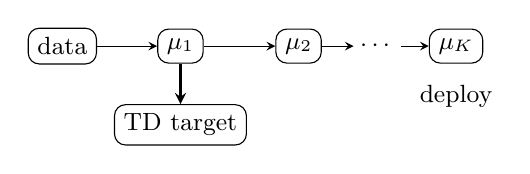
\begin{tikzpicture}[x=1cm,y=1cm,>=stealth,every node/.style={font=\small}]
\node[draw,rounded corners] (d) at (0,0) {data};
\node[draw,rounded corners] (a1) at (1.5,0) {$\mu_1$};
\node[draw,rounded corners] (a2) at (3.0,0) {$\mu_2$};
\node at (4.0,0) {$\cdots$};
\node[draw,rounded corners] (ak) at (5.0,0) {$\mu_K$};
\node[draw,rounded corners] (td) at (1.5,-1.0) {TD target};
\draw[->] (d)--(a1); \draw[->] (a1)--(a2); \draw[->] (a2)--(3.7,0); \draw[->] (4.3,0)--(ak); \draw[->,thick] (a1)--(td);
\node[below=.15cm of ak] {deploy};
\end{tikzpicture}
\caption{BAR routes only the first actor into Bellman targets and deploys the last actor.}
\label{fig:routing}
\end{figure}

\subsection{A simpler separation control}
The direct two-actor control removes sequential re-centering. Both actors are anchored directly to dataset actions. For the P4 comparison, the target actor uses nominal coefficient $T/4$ and alone enters Bellman backups, while the deployed actor uses coefficient $T$. This is a mechanism control inspired by target/evaluation separation; it is not a reproduction of published MCEP.

\subsection{Finite-step statements}
For deterministic policies and state distribution $\rho$, define
\begin{equation}
\mathsf d_{d,\rho}^2(\mu,\nu)=\E_{s\sim\rho}\frac{\|\mu(s)-\nu(s)\|_2^2}{d}.
\end{equation}
Since $W_2^2(\delta_{\mu(s)},\delta_{\nu(s)})=\|\mu(s)-\nu(s)\|^2$, the TD3+BC anchor is a rescaled integrated squared Wasserstein distance. With fixed normalized critic, the ideal proximal map is
\begin{equation}
\mathcal P_h^{\bar Q}(\nu)\in\argmin_\mu\left\{-\E_s\bar Q(s,\mu(s))+\frac{1}{2h}\mathsf d_d^2(\mu,\nu)\right\}.
\end{equation}
The live implementation takes only one Adam step and later persistent actors need not approach the identity as $h\to0$; this ideal map motivates but does not certify the trained chain.

\begin{proposition}[First-hop target perturbation]
Suppose each $Q_j^-(s',\cdot)$ is $L(s')$-Lipschitz. For a reference policy $\mu_0$,
\begin{equation}
\|y_{\mu_1}-y_{\mu_0}\|_{L_2(\D)}\le\gamma\left(\E_{s'}L(s')^2\|\mu_1(s')-\mu_0(s')\|_2^2\right)^{1/2}.
\end{equation}
Conditional on $\mu_1$, later actors do not enter this one-step difference.
\end{proposition}
This is an architectural bound, not a critic-stability theorem. We therefore use \emph{bootstrap exposure} operationally for target-action displacement and separately audit the realized TD-target value difference.

\section{Experiments}
We evaluate on the nine D4RL locomotion tasks formed by Hopper, HalfCheetah, and Walker2d with medium, medium-replay, and expert datasets \citep{fu2020d4rl}. Scores are D4RL normalized returns. The main sweep uses fourteen budgets
\[
T\in\{.05,.1,.2,.4,.7,1.5,2.5,4,7,10,12,14,17,20\}
\]
and four seeds for each headline depth. Every score is the ten-episode mean at one million critic updates. The high-budget estimand first averages seeds and the seven $T\ge4$ values within task and then weights the nine task variants equally. A seed-mean task--budget cell below score 20 is descriptively called collapsed.

\subsection{Depth broadens the BAR stability envelope}
\begin{table}[t]
\caption{Four-seed fixed-budget results. High: $T\ge4$; Tail: $T\ge10$. Collapse: seed-mean cells / raw seeded runs at score $<20$.}
\centering\small
\setlength{\tabcolsep}{3pt}
\begin{tabular}{lrrrr}
\toprule
Method & $T\le2.5$ & High & Tail & Collapse\\
\midrule
TD3+BC &66.68&25.38&20.27&34 / 142\\
BAR-P2 &70.64&41.20&31.01&22 / 111\\
BAR-P3 &70.53&51.92&42.23&16 / 84\\
BAR-P4 &\textbf{70.82}&\textbf{63.97}&\textbf{56.79}&\textbf{8 / 54}\\
BAR-L2 &69.79&38.43&28.47&25 / 112\\
BAR-L3 &69.73&46.44&35.83&21 / 95\\
\bottomrule
\end{tabular}
\label{tab:depth}
\end{table}
The proximal ordering is reproduced by both disjoint seed pairs. The P4--P3 high-budget gain is $12.06$ with task-resampling interval $[3.84,21.11]$, but the cellwise median is only $+0.34$: eight severe rescues account for most of the aggregate gain. The projected-linearized realization also improves from L2 to L3 by $8.01$ points, so the depth phenomenon is not unique to the proximal loss.

The result is not confined to an artificial stress tail. TD3+BC's descriptive grid maximum is $74.79$, while BAR-P4 reaches $82.06$. Nevertheless, the paper does not provide an offline rule for selecting $T$ or $K$.

\subsection{Movement and critic failure signatures}
On 90 matched high-budget cells for seeds 0--1, BAR-P3 has lower deterministic next-state target-action displacement than TD3+BC in $88/90$ comparisons (median ratio $.658$), while its current-state final-policy displacement is lower in only $36/90$ (median ratio $1.057$). P4 lowers target displacement in $89/90$ matched comparisons with TD3+BC. Thus moderate BAR can reduce the movement entering bootstrapping without simply shrinking the evaluated actor.

Collapsed runs exhibit orders-of-magnitude larger TD-error tails and critic magnitudes. Under a frozen common critic, median actor-path gain changes sign between stable and collapsed runs, and a targeted simulator-reference audit finds extreme positive critic miscalibration in collapsed checkpoints. These diagnostics are consistent with critic failure, but they do not make target displacement a sufficient predictor of return.

A separate verified 270-checkpoint audit directly computes the same-noise RMS change in target values under target-actor versus paired dataset actions and evaluates first/final geometry on the same next-state batch. The audit retains large finite tails rather than filtering them. Its role is diagnostic: target-value perturbation depends jointly on action displacement and critic sensitivity, and neither quantity alone determines return.

\subsection{The decisive controls favor separation over a chain-specific claim}
The first broad control compares BAR-P3 with two directly data-anchored actors: target coefficient $T/3$, deployment coefficient $T$. Over 90 matched pairs, the two-actor control scores $59.22$ versus $57.67$ for the contemporaneous BAR-P3 rerun; both have $9/45$ seed-mean score-$<20$ cells. Control minus BAR has interval $[-1.52,5.44]$. Sequential re-centering is therefore not required to reproduce the P3 aggregate regime.

We then prelocked a P4 comparison over nine tasks, $T\in\{4,7,10,14,20\}$, and seeds 0--1. Both procedures were rerun contemporaneously. The primary contrast is BAR-P4 deployment minus two-actor-P4 deployment.
\begin{table}[t]
\caption{Locked P4 procedure comparison over 90 task--budget--seed pairs. The primary continuous result is unresolved by the predeclared decision rule.}
\centering\small
\begin{tabular}{lr}
\toprule
Statistic & BAR $-$ two-actor\\
\midrule
Task-equal mean & $-2.31$\\
95\% task-resampling interval & $[-7.25,\ 2.41]$\\
Paired median & $+0.68$\\
Wins / ties / losses & $55/1/34$\\
Score-$<20$ raw runs & $12$ vs. $11$\\
Score-$<20$ seed-mean cells & $5$ vs. $3$\\
\bottomrule
\end{tabular}
\label{tab:p0}
\end{table}
The mean and median have opposite signs because both procedures show heavy-tailed task/seed failures. Task means range from $-13.45$ (Walker2d-medium) and $-12.41$ (Hopper-expert) to $+9.88$ (Walker2d-medium-replay). The predeclared minimum worthwhile difference was three points: a procedure-supporting label required a 95\% interval wholly on one side of zero and a point estimate of at least three points in magnitude; practical comparability required the full interval to lie in $[-3,3]$. None holds, so the locked label is \emph{unresolved}. Importantly, there is no evidence here that the four-actor chain supplies an additional stability advantage over direct target/deployment separation.

The score archive is a frozen cross-host merge of all 180 finals. At the time of this draft, the score-level statistics are complete while the single-host checkpoint-bound analyze/verify receipt for all 180 runs is not available; we therefore treat the P0 result as scientifically informative but preserve this provenance limitation.

\subsection{Local theory scope and cost}
For a learned ReLU critic, the action gradient is piecewise constant within a fixed activation region. A verified audit on 6144 Hopper/Walker anchors measures full-region residence $0.954,0.911,0.842,0.748$ at local horizons $T=.025,.05,.1,.2$. This supports only the local affine scope of the explicit/implicit interpretation; it is not evidence for a global proximal solution or for the live chain.

BAR stores $K$ actors and makes $K$ actor optimizer calls per delayed update. On one H200/JAX 0.10.2 stack, measured compiled actor-phase time increases from $1.435$ ms at $K=1$ to $1.887$ ms at $K=4$, while the scoped backend high-water memory increases from $9.68$ MB to $18.05$ MB. These are one-stack measurements rather than end-to-end training costs.

\section{Discussion}
The experiments separate three claims that are easy to conflate. First, \emph{within BAR}, increasing depth strongly broadens the observed stability envelope. This end-to-end fact is robust across four seeds and two actor realizations. Second, BAR produces the intended architectural geometry: the first branch can move less while the deployed branch retains reach. Third, the controls do \emph{not} show that predecessor re-centering or a $K$-actor chain is necessary for the return improvement. Direct two-actor separation reaches the same P3 aggregate and remains statistically unresolved against P4.

The safest mechanistic conclusion is therefore role separation, not chain superiority. A conservative bootstrap branch reduces the immediate movement presented to Bellman regression, while an independently stronger deployment branch preserves policy improvement. This is compatible with the first-hop perturbation bound and with the observed movement audits, but it is not a proof that lower exposure causes higher return. Critic sensitivity, optimization history, projection, and training-seed bifurcation remain important.

This reframing also clarifies the relation to MCEP. The broad two-policy principle has precedent; BAR contributes a controlled depth probe and an unusually dense stability/failure characterization. The P0 result is useful precisely because it prevents over-attributing the gain to the sequential chain.

\paragraph{Limitations.}
The benchmark has only three dynamics families and all experiments use a TD3+BC backbone. Task-resampling intervals therefore describe variation over this fixed benchmark rather than broad offline-RL generalization. Some historical seed-2/3 run manifests were not retained. The P0 score merge spans two hosts and lacks a unified checkpoint-bound verification receipt. Collapse thresholds are descriptive. No offline selection rule chooses $T$ or $K$. Finally, target-action displacement and target-value perturbation are mechanism readouts, not causal certificates of critic reliability or environment return.

\section{Conclusion}
Budgeted actor refinement reveals a clear empirical fact: offline actor--critic training becomes much more robust to aggressive policy-improvement coefficients when the actor branch exposed to Bellman bootstrapping is separated from the branch used for deployment. BAR's depth sweep expands the stability envelope dramatically, but the decisive controls revise the interpretation: sequential re-centering is not established as necessary, and a simpler directly data-anchored two-actor procedure remains competitive at both P3 and P4. The main design principle is therefore target--deployment decoupling. BAR is best understood as a strong routed procedure and a depth-indexed probe of that principle, rather than as evidence that additional proximal hops are intrinsically superior.

\bibliography{references}
\section*{Checklist}

\begin{enumerate}
\item For all models and algorithms presented, check if you include:
  \begin{enumerate}
  \item A clear description of the mathematical setting, assumptions, algorithm, and/or model. [Yes/No/Not Applicable]\\
  \textbf{Yes.} The main paper defines the offline MDP setting, TD3+BC backbone, BAR actor chain, routing, direct two-actor control, and the distinction between the ideal proximal map and the live one-Adam-step implementation.
  \item An analysis of the properties and complexity (time, space, sample size) of any algorithm. [Yes/No/Not Applicable]\\
  \textbf{Yes.} BAR stores $K$ persistent actors and makes $K$ actor optimizer calls per delayed update. The paper reports both the $O(K)$ actor-work scaling and one-stack H200 timing/memory measurements for $K=1$ and $K=4$.
  \item (Optional) Anonymized source code, with specification of all dependencies, including external libraries. [Yes/No/Not Applicable]\\
  \textbf{Partial.} The release contains BAR, the two-actor control, diagnostic runners/verifiers, compact scientific artifacts, and dependency files. Some historical runs predate the current provenance harness and therefore lack a complete executable historical snapshot.
  \end{enumerate}

\item For any theoretical claim, check if you include:
  \begin{enumerate}
  \item Statements of the full set of assumptions of all theoretical results. [Yes/No/Not Applicable]\\
  \textbf{Yes.} The first-hop target-perturbation result states its Lipschitz assumption; the Wasserstein/proximal and local explicit--implicit statements are explicitly restricted to deterministic policies, fixed critics/scales, and local conditions where appropriate.
  \item Complete proofs of all theoretical results. [Yes/No/Not Applicable]\\
  \textbf{Yes.} The supplementary material gives the behavior-anchor decomposition, inexact learned-critic margin, target-perturbation proof, and local explicit--implicit expansion.
  \item Clear explanations of any assumptions. [Yes/No/Not Applicable]\\
  \textbf{Yes.} The paper repeatedly distinguishes ideal fixed-critic statements from the persistent neural actor chain and reports a learned-ReLU activation-region residence audit to delimit the local interpretation.
  \end{enumerate}

\item For all figures and tables that present empirical results, check if you include:
  \begin{enumerate}
  \item The code, data, and instructions needed to reproduce the main experimental results (either in the supplemental material or as a URL). [Yes/No/Not Applicable]\\
  \textbf{Yes.} The repository contains fixed score matrices, compact diagnostic CSV/JSON artifacts, analysis/verifier code, experiment runbooks, and manuscript build instructions. Public D4RL datasets are cited.
  \item All the training details (e.g., data splits, hyperparameters, how they were chosen). [Yes/No/Not Applicable]\\
  \textbf{No.} All recoverable algorithmic settings are documented, but exact historical per-run manifests for proximal seeds 2--3 were not retained, and the exact historical Git revision of the earlier P3 two-actor control was never persisted. New locked experiments retain substantially stronger provenance.
  \item A clear definition of the specific measure or statistics and error bars (e.g., with respect to the random seed after running experiments multiple times). [Yes/No/Not Applicable]\\
  \textbf{Yes.} The paper defines the four-seed score grids, task-equal high-budget estimand, raw and seed-mean collapse counts, task-resampling intervals, paired P0 contrast, movement ratios, target-value RMS diagnostic, and the resampling/generalization scope.
  \item A description of the computing infrastructure used. [Yes/No/Not Applicable]\\
  \textbf{Partial.} The measured actor-cost audit records an H200/JAX 0.10.2 stack and new locked experiments record host/accelerator inventories. A complete independently verified hardware inventory for every historical headline run was not retained.
  \end{enumerate}

\item If you are using existing assets (e.g., code, data, models) or curating/releasing new assets, check if you include:
  \begin{enumerate}
  \item Citations of the creator if your work uses existing assets. [Yes/No/Not Applicable]\\
  \textbf{Yes.} D4RL, TD3+BC, CORL, and the relevant prior methods are cited.
  \item The license information of the assets, if applicable. [Yes/No/Not Applicable]\\
  \textbf{Yes.} The released repository identifies its license; upstream packages and benchmark assets retain their respective licenses.
  \item New assets either in the supplemental material or as a URL, if applicable. [Yes/No/Not Applicable]\\
  \textbf{Yes.} Compact P0--P3 evidence, verification receipts where available, and analysis code accompany the source release.
  \item Information about consent from data providers/curators. [Yes/No/Not Applicable]\\
  \textbf{Not Applicable.} The work uses public simulated-control benchmark data and no human-subject data.
  \item Discussion of sensitive content if applicable. [Yes/No/Not Applicable]\\
  \textbf{Not Applicable.} The assets contain simulated locomotion trajectories and no personal or sensitive information.
  \end{enumerate}

\item If you used crowdsourcing or conducted research with human subjects, check if you include:
  \begin{enumerate}
  \item The full text of instructions given to participants and screenshots. [Yes/No/Not Applicable]\\
  \textbf{Not Applicable.}
  \item Descriptions of potential participant risks, with links to Institutional Review Board approvals if applicable. [Yes/No/Not Applicable]\\
  \textbf{Not Applicable.}
  \item The estimated hourly wage paid to participants and the total amount spent on participant compensation. [Yes/No/Not Applicable]\\
  \textbf{Not Applicable.}
  \end{enumerate}
\end{enumerate}

\end{document}
